
\mysection{Introduction}

Vu de l’extérieur, un manipulateur robotique polyvalent pourrait sembler être une technologie plutôt inoffensive, pas très différent d’un tapis roulant ou d’une perceuse, mais l’aspect innovant de ce type de machines est précisément sa polyvalence. Étant reprogrammable, le manipulateur n’est pas limité à une utilisation particulière, ce qui veut dire que le fabricant n’a pas besoin de traiter des considérations particulières d’une industrie donnée, mais seulement avec des aspects généraux (vitesse maximale, couple maximal, déplacement maximum, etc). Le but de ce travail est précisément d’explorer cet aspect polyvalent d’un manipulateur en proposant un système qui permet à l’utilisateur de commander la position de l’extrémité du manipulateur et ses trajectoires. On proposera une application simple pour ce système, dont le but est de démontrer son fonctionnement et évaluer ses performances. Le système complet est schématisé sous la
forme simplifiée ci-dessous: 

\begin{figure}[H]
	\begin{center}	
		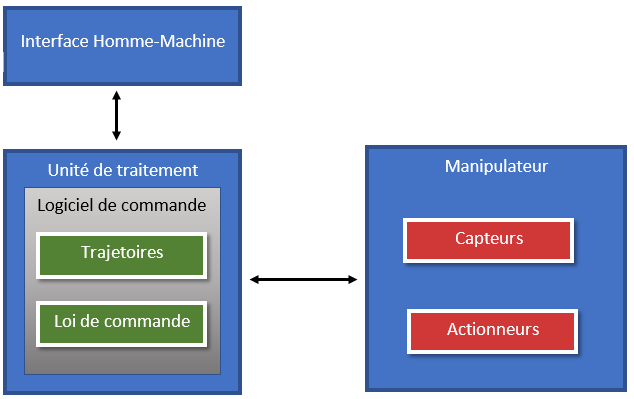
\includegraphics[width=10cm]{./IntroImage}
		\caption{Schéma simplifié du système.}
		\label{fig:Schema}
	\end{center}
\end{figure}